%!TEX root = thesis.tex
\chapter{2-D Imaginary Time Evolving Block Decimation}
\label{chapter:2ditebd}

In this chapter we introduce some different ways to implement two-dimensional imaginary time-evolving block decimation and apply them in calculation of ground state of Heisenberg and transverse Ising model on two-dimensional square lattice. In section \ref{ite} and \ref{itebd}, we briefly review the idea of imaginary time evolution (iTEBD),[\ref{vidal}] and explain how to extend it to two-dimensional [\ref{X,zhon}]. Second, we briefly review another method to make 2D-iTEBD more stable[\ref{1.1}]. In the last section \ref{2dopt}, we record various particulars which are helpful optimizing algorithms.

\section{Imaginary Time Evolution}
\label{ite}
Theoretically, if having the imaginary time evolution operator $e^{-\tau H}$, we could project any random states to the ground state, as long as the wave-function can be written as,
\begin{align}
	\label{mapgroud}
	\Ket{\psi_0} = \frac{e^{\tau H} \Ket{\Psi}}{\parallel e^{\tau H} \Ket{\Psi}\parallel}
\end{align}
but according to the eq.\ref{mapgroud}, we may found that the number of coefficients in an origin evolution operator $e^{-\tau H}$ is proportional to $2^N \times 2^N$. On the other words, it is impossible to update entire system directly. In order to restricting the rapid dimensional growth, we apply \textit{Suzuki Trotter decomposition}[\ref{1.1}][\ref{1.1}] to approximate. The main idea of \textit{Suzuki Trotter} is decomposing the whole system to lots of units cell and using some smaller operations to update the wave-function.
\begin{align}
	\label{STd}
	e^{\delta A + B} = e^{\delta A}e^{\delta B} + O(\delta^2)
\end{align}
eq.\ref{STd} means the first-order Suzuki Trotter  decomposition, and A and B are non-commutative with each other.

Now that the dimension of the evolution operator is reduced to a n-site operator and in chapter \ref{chapter:properties}, we have shown that a many-body system can map to a MPS or PEPS structure, so we can draw the process of updating a ground state like Fig.\ref{fig312},

\begin{figure}[ht]
	\centering
	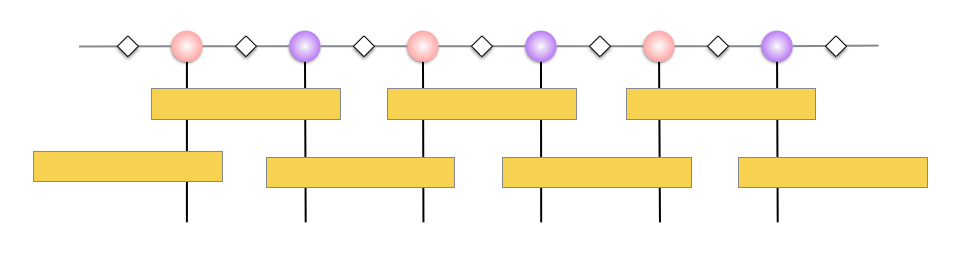
\includegraphics[width=0.75\textwidth]{figures/fig312.png}
	\caption[The picture of the main idea of itebd.]{The red and blue tensor denotes on \textit{odd} and \textit{even} sites. The yellow one are time evolution operators $e^{-\tau H_{k,k+1}}$, $e^{-\tau H_{k+1,k}}$}
	\label{fig312}
\end{figure}

On the other work, contract the tensors in Fig.\ref{fig312} repeatedly until the ground state energy to the minimum. The remained tensor is considered as the ground state of the system. So the next question: How can we contract them and preserve the structure like Fig{\ref{fig311}}? This answer is iTEBD.

\begin{figure}[ht]
	\centering
	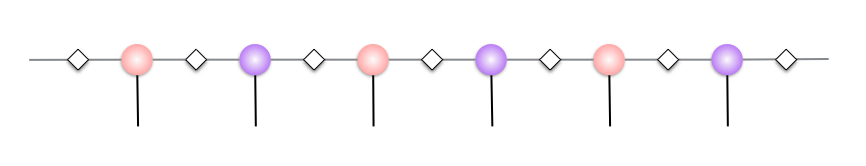
\includegraphics[width=0.75\textwidth]{figures/fig311.png}
	\caption[The picture of matrix product states]{The simple form of a matrix product state.}
	\label{fig311}
\end{figure}

\section{Infinite Imaginary-Time Evolving Block Decimation}
\label{itebd}
\subsection{D = 1}
\label{1ditebd}
	\begin{figure}[ht]
	\centering
	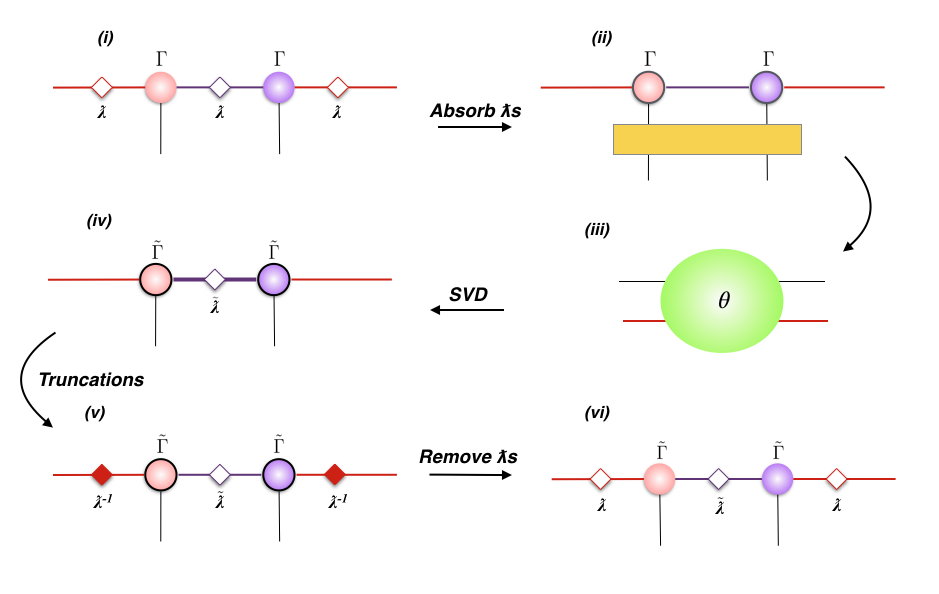
\includegraphics[width=0.75\textwidth]{figures/fig313.png}
	\caption[tmp]{}
	\label{fig313}
	\end{figure}

\subsection{D = 2}
\label{2ditebd}
	\begin{figure}[ht]
	\centering
	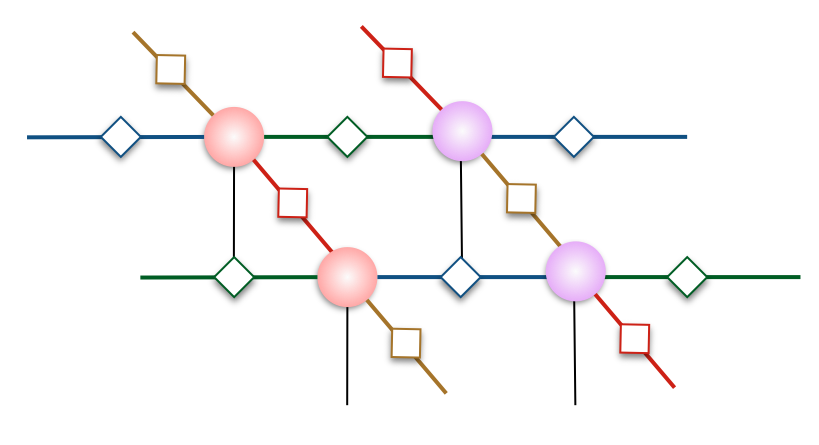
\includegraphics[width=0.75\textwidth]{figures/fig314.png}
	\caption[tmp]{}
	\label{fig314}
	\end{figure}

	\begin{figure}[ht]
	\centering
	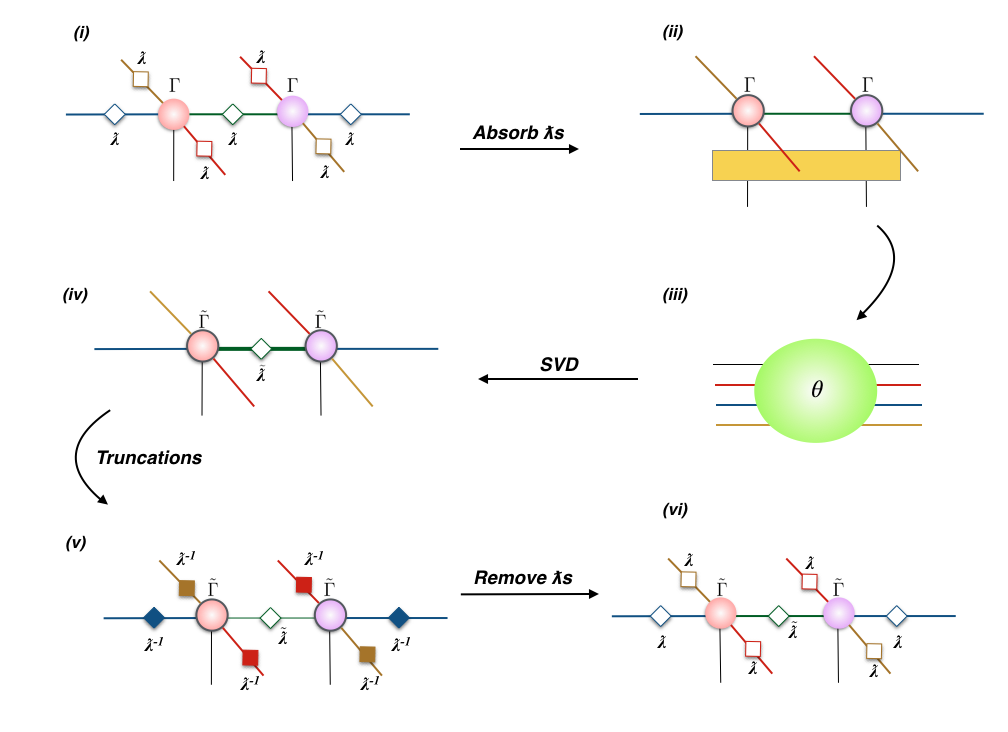
\includegraphics[width=0.75\textwidth]{figures/fig315.png}
	\caption[tmp]{}
	\label{fig315}
	\end{figure}

\section{Ameliorate two-dimensional iTEBD}
\label{2dhastin}

	\begin{figure}[ht]
	\centering
	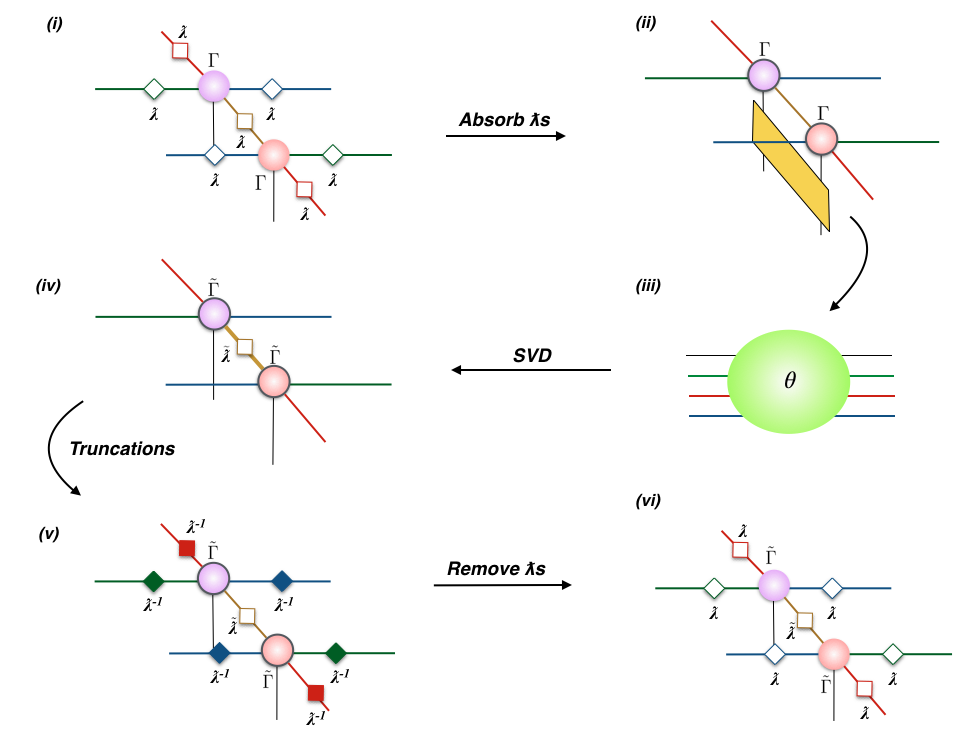
\includegraphics[width=0.75\textwidth]{figures/fig316.png}
	\caption[tmp]{}
	\label{fig316}
	\end{figure}

\section{Optimizations}
\label{2dopt}

\subsection{QR decomposition}
\label{2doptQR}
	\begin{figure}[ht]
	\centering
	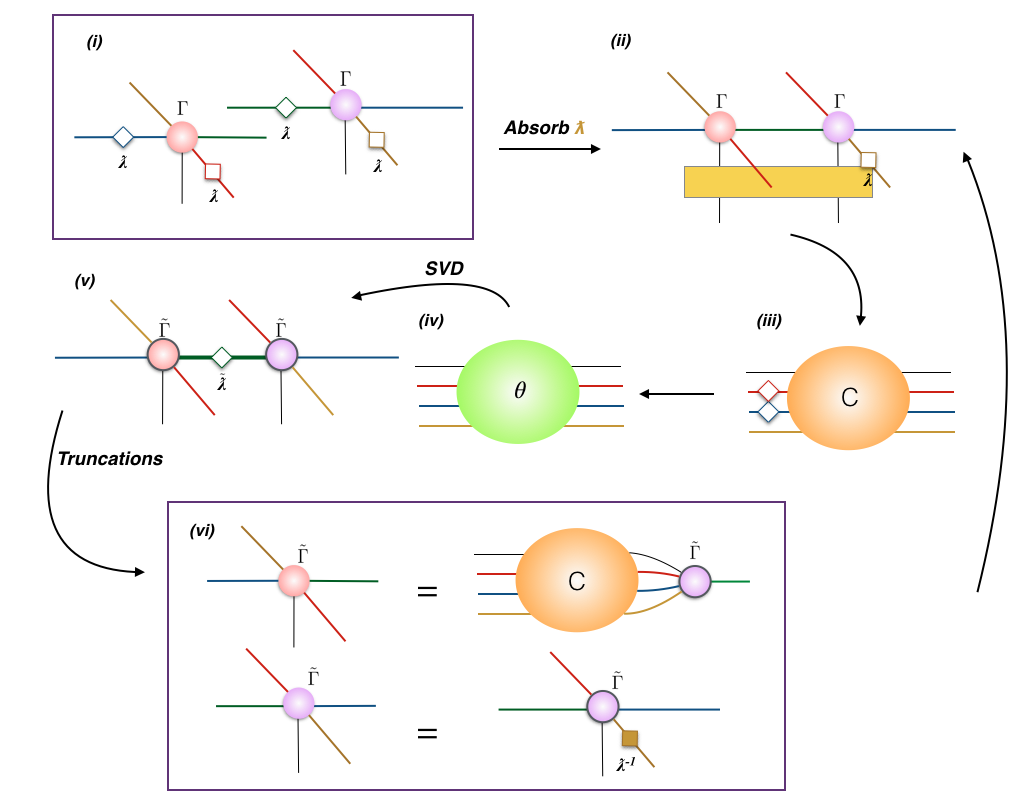
\includegraphics[width=0.75\textwidth]{figures/fig317.png}
	\caption[tmp]{}
	\label{fig317}
	\end{figure}

	\begin{figure}[ht]
	\centering
	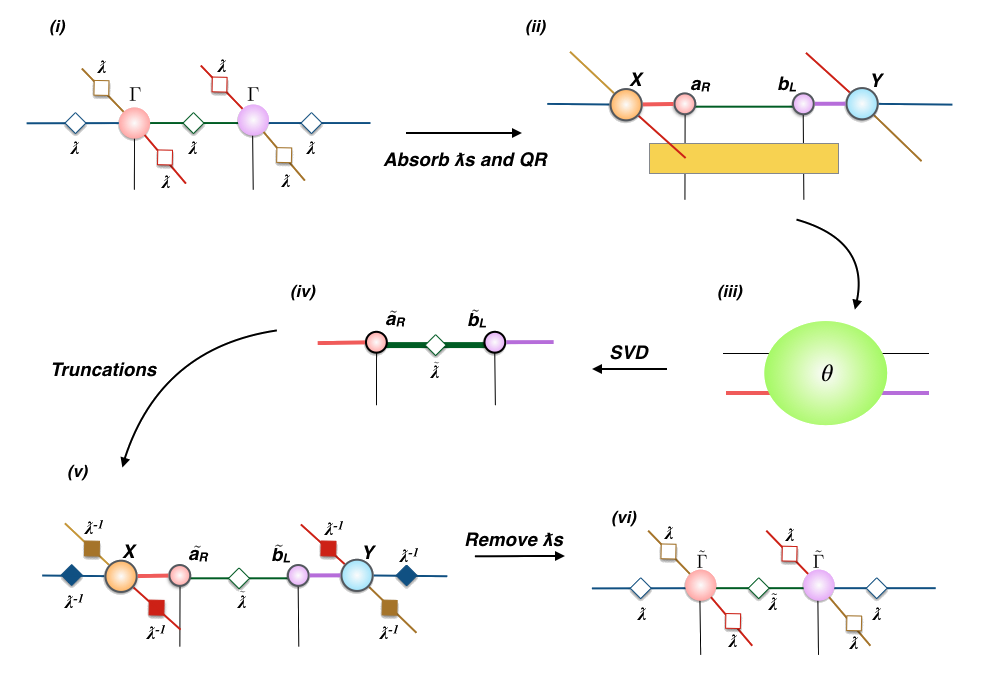
\includegraphics[width=0.75\textwidth]{figures/fig318.png}
	\caption[tmp]{}
	\label{fig318}
	\end{figure}

	\begin{figure}[ht]
	\centering
	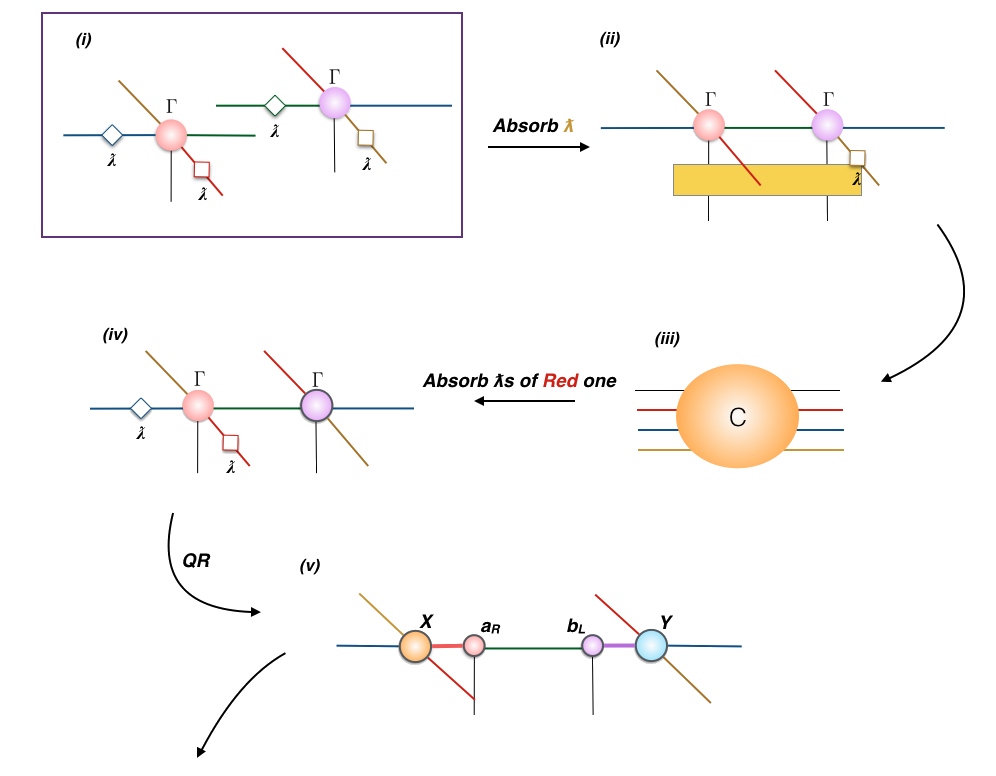
\includegraphics[width=0.75\textwidth]{figures/fig319.png}
	\caption[tmp]{}
	\label{fig319}
	\end{figure}

\subsection{Initialization}
\label{2doptInit}

